\section{Architecture}

Modern computer science emphasize parallelism as a highly important property in
order to achieve speed on multicore processors. As the size of the log files
which PET has to parse can easily be 10s of gigabytes large, PET has to be
designed with performance in mind. This means that PET must be lightweight and
parallel in order to be fast, while it must maintain correctness and be easy to
use.

Due to memory constraints on commonly available computers, it is not feasible to
read the entire log file into memory and then start parsing. It would also make
the reading step a serial part of the program, which hinders parallelism. It
will also be a bad idea to read one line, parse it, weight it and apply it to
the grand total, as it would be an entirely serial process.

\subsection{Overview}

\begin{figure}[ht]
    \includegraphics[width=0.9\textwidth]{figs/pet-pipeline-gv.pdf}
    \caption{How PET works}
    \label{fig:pipeline}
\end{figure}

In order to maintain good speed while still keeping the PET source code
readable, we have looked at different ways of chewing through large data sets.
The final implementation of PET follows a scheme borrowing ideas from the
producer-consumer patterb as explained by Gamma et. al. in \cite{designpatterns}
and the MapReduce algorithm \cite{dean2008mapreduce}. As depicted in
\autoref{fig:pipeline}, this scheme makes it rather easy to let a producer read
the lines from the log file into ring buffers (produce) and let multiple
consumers pick from each their ring buffer (consume). Each consumer parses the log
lines they pick, and apply the weight of each read event to each their result
vector (map). When all lines are read and parsed, the results vectors are
merged, and idle-task power and static power consumption is added (reduce). This
combination of algorithms allows PET to take advantage of as many cores as
possible, limted only by how fast the producer can read the log files. Finally,
a human readable output is produces, either as a gnuplot line graph or as
formatted or plain text output.

The next subsections will describe in detail the most imporatant parts of the
workflow. For further understanding of the program flow, a call graph extracted
from the entire source code can be found in \autoref{fig:callgraph}.

\begin{figure}
    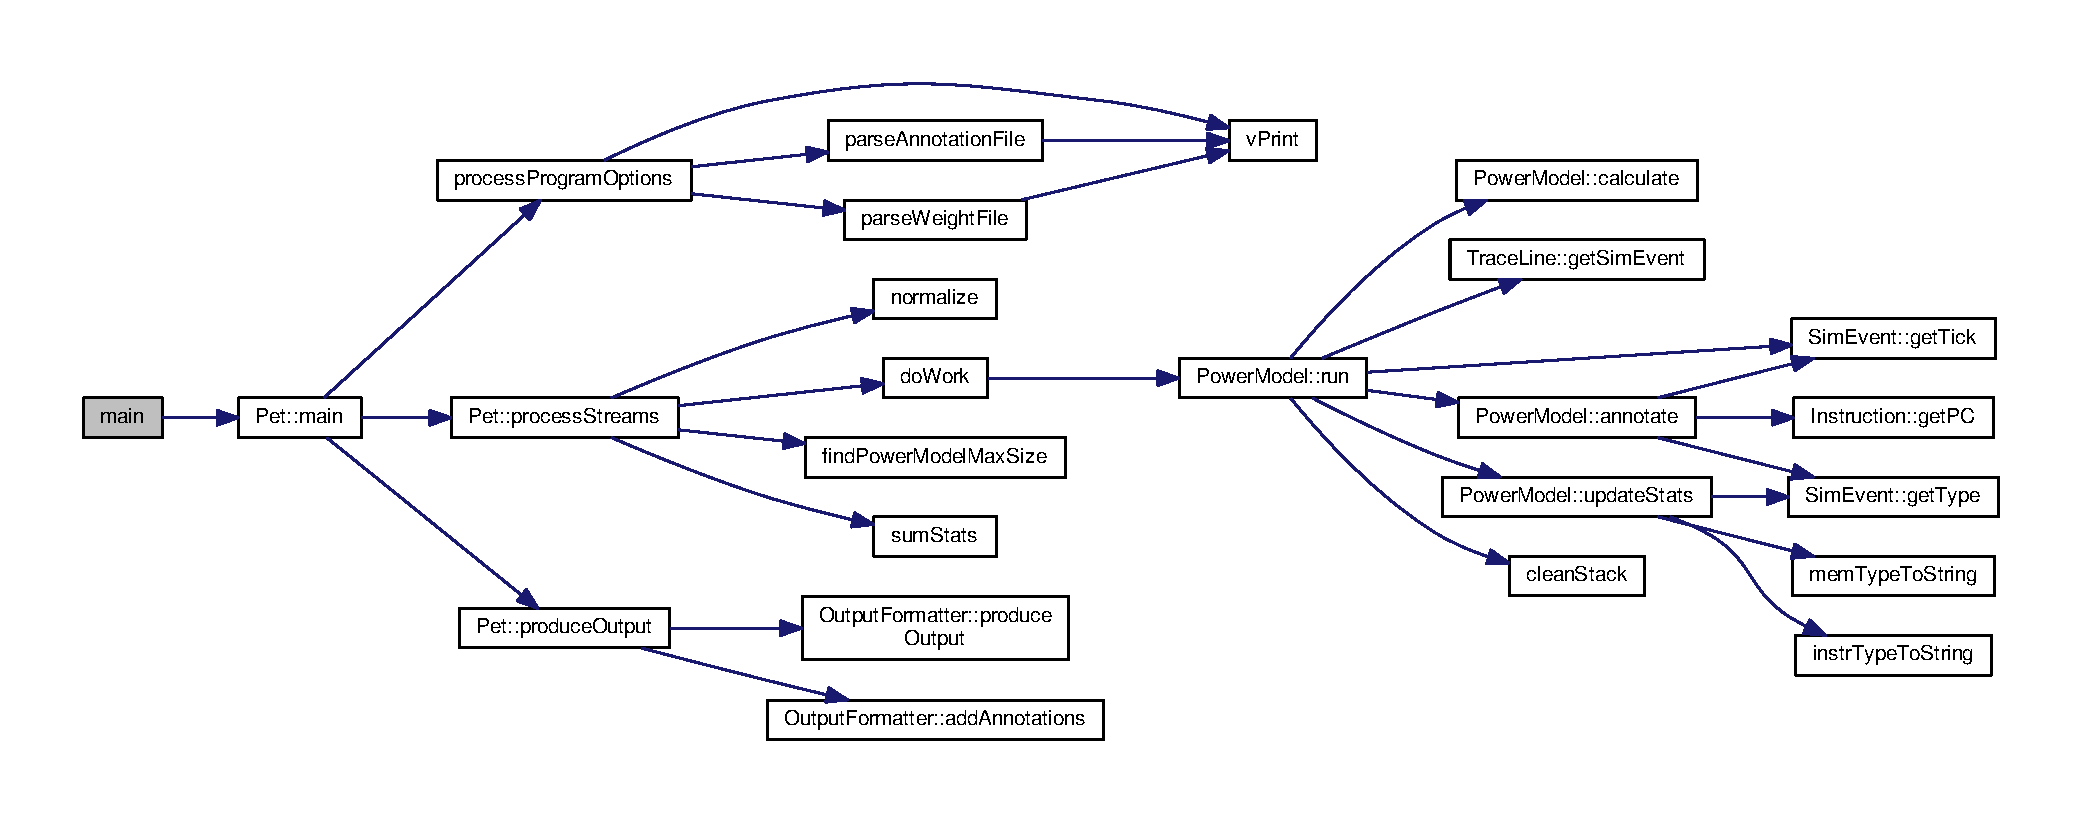
\includegraphics[width=\textwidth]{figs/maincallgraph.pdf}
    \caption{Call graph}
    \label{fig:callgraph}
\end{figure}



\subsection{Argument Parsing and Program Options}

As any other non-trivial programs, PET has to adapt to input options given from
the command line or from a settings-file. PET makes extensive use of the
\texttt{Boost}-library \cite{boostwebpage} and utilize
\texttt{Boost::Program\_options} for parsing the command line. Making use of
\texttt{Boost} for common tasks all over the program made the development cycle
less cumbersome and more rapid. \texttt{Boost::Program\_options} allows easy
extraction of program options, both with long (\texttt{\textemdash \textemdash
option=\emph{value}}) and short (\texttt{\textemdash o~\emph{value}})option
style.


\subsection{Reading Trace Logs}

When arguments are parsed and a trace log has been specified, either by path or
as \texttt{stdin}, a single thread is kicked off reading each line of the log
file into a C++ string container. This happens in the
\texttt{Pet::processStreams} method seen in \autoref{fig:callgraph}. The string
container is then inserted into one of many circular buffers. The circular
buffers are implemented with \texttt{boost::lockfree::spsc\_queue}, a lock free
single producer, single consumer queue. The property of beeing lock free is
explained by Tim Blechmann and the boost-community in \cite{boostlockfree} as
follows: "data structures are \emph{lock-free}, if some concurrent operations
are guaranteed to be finished in a finite number of steps. While it is in theory
possible that some operations never make any progress, it is very unlikely to
happen in practical applications". In PET, this queue has a fixed size of 8192,
but dynamic size is also available in the library implementation.

Which buffer the string is inserted into is determined by a simple circular
algorithm; the next ring buffer is selected when current one is full. When the
buffers are small enough to be filled fast enough to let all workers do work,
this method creates a lot less locking than using a single ring buffer shared by
all worker threads. The number of threads and the size of the ring buffers are
tightly coupled with how fast the host computer is able to feed PET with the log
files.

It is our experience that reading the log file is not the bottle neck, and it is
easy to feed at least 8 cores when the log file is hosted on a reasonable fast
drive. A simple benchmarking done with PET running on a system consisting of an
Intel Core i7 4820, 32GB DDR3 SDRAM and keeping the log files on a fake-RAID
Level-0 consisting of two Western Digital Caviar Black 750GB disks shows this.
PET running with 8 threads on this particular system is consuming the log files
with a rate of 133MB/s regardless of where the log files resides in RAM or on
disk. The benchmark used a log file of 5458MB and was run in 40.871 seconds.

\subsection{String to Event Mapping and Power Accumulation}

String parsing and mapping resembles the most compute-intensive parts of PET.
These parts of the program is kicked off as thread starting the
\texttt{doWork}-function, as the thread library cannot start running in methods
of instanceiated objects. As displayed in the callgraph in
\autoref{fig:callgraph}, this function simply starts the
\texttt{PowerModel::run}-method on it's input, which an instance of the
PowerModel-class.

As the producer fills the ring buffers for each of the workers, the workers pick
strings from their pool. The strings are popped from the ring buffer, thus
making space for new elements right away. Each string is parsed by the TraceLine
class, which looks for patterns in the strings containing known event types.
When connecting PET with gem5, the trace logs as previously seen
\autoref{lst:trace} contains an event type designation in the second :-separated
column. The TraceLine class extracts this part using a very simple method to
make this part go fast, outline of this method is listed in
\autoref{alg:extract}.

\begin{algorithm}
    \begin{lstlisting}[style=algo,language=python]
function extractEventType( line ):
    start = line.find(":") + 1
    end = line.find(":", start)

    while (line[start] == ' ')
        start = from + 1
    while (line[end-1] == ' ')
        end = to - 1

    return line.substring(start, end)
    \end{lstlisting}
    \caption{Event Type Extraction}
    \label{alg:extract}
\end{algorithm}

In the real program, some more error handling is present, and the event types
are instanceiated as objects of their parent type (Instruction- or
Memory-event). The right parameters are further found from progressive string
parsing. If the event is not recognized, an "empty" object of type UnknownEvent
is returned, this type always has zero weight. Each event object is able to
figure out it's own weight as written in the \emph{weights}-file. After the
event has been parsed, it's weight is added to the power model at the right
time step.

In order to reduce the time used for disposal of the string objects
after they are parsed, they are places in a static-size array. When
this array is full, or the ring buffer is empty, the worker deletes
all the strings in a chunk. This methods keeps the memory footprint
low while not calling \texttt{free()} at a continuous rate. The \texttt{free()}
function is not considered very slow, but from the reference implementation
shown in \cite{kernighan1988c}, it does contain enough pointer
arithmetics to make a difference in a tight loop.

\subsection{Data Reduction}

When all lines from the trace log are consumed by the workers, the threads are
joined and their data is contained as standard C++-vectors in a standard
C++-vector. The inner vectors is looped over together, and the value from the
current data point in each vector is added together and put in a result vector.
This work is done as the last part of \texttt{Pet::processStreams} as seen in
\autoref{fig:callgraph}. After a single point has been accumulated from the
vectors, idle time is calculated from how many events that was recorded during
the data point. This is done more simplistic than accurate using
\autoref{eq:idle}. $numEvents$ is the number of events recorded in each vector
at each measure point, and each event is pinned to the cycle where it
originated.

\begin{equation}
    totalEvents = \sum_{n=1}^{N} numEvents_n
\end{equation}
\begin{equation}
    idleEvents = \frac{ticksInDatapoint}{ticksInCycle}- totalEvents
\label{eq:idle}
\end{equation}



\subsection{Output Production and Annotations}



\subsection{Unit Tests}


